\documentclass[a4paper,addpoints,12pt]{exam}

\usepackage{dlds}

\usetikzlibrary{arrows}

 
\begin{document}

\devoir[prv=false,ds=true,num=2 ,niv=3 , date=12/12/2022 ]
\begin{exo}[3]
\begin{minipage}{.5\linewidth}
$a$ et $b$ sont deux nombres réels tels que $a\leq b$

Comparer $a$ et $\dfrac{a+b}{2}$
\end{minipage}
\begin{minipage}{.5\linewidth}
\notes[10pt]{3}{\textwidth}
\end{minipage}
\end{exo}

\begin{exo}[8]
$a$ et $b$ sont deux nombres réels tels que $4\leq a\leq 7$ et $-8\leq b\leq -1$
\begin{questions}
\question Encadrer $2a+3b$ et $a-b$ et $ab$ et $\dfrac{a}{b}$
\question Sachant que $2\leq \sqrt{6}\leq 3$ et $1.7\leq \sqrt{3}\leq 1.8$.Encadrer $\sqrt{18}$ et $\sqrt{2}$
\end{questions}
\end{exo}

\begin{exo}[9]
\begin{minipage}{0.4\linewidth}
\definecolor{cqcqcq}{rgb}{0.7529411764705882,0.7529411764705882,0.7529411764705882}
\begin{tikzpicture}[line cap=round,line join=round,>=triangle 45,x=1.0cm,y=1.0cm]
\clip(-2.92,-1.84) rectangle (3.22,5.62);
\draw [domain=-2.92:3.22] plot(\x,{(-6.-3.*\x)/-2.});
\draw [domain=-2.92:3.22] plot(\x,{(--1.68-4.06*\x)/0.56});
\draw (-2.,0.)-- (0.56,-1.06);
\draw [domain=-2.92:3.22] plot(\x,{(--1.724615384615385-1.06*\x)/2.56});
\draw [dash pattern=on 5pt off 5pt,domain=-2.92:3.22] plot(\x,{(--12.575915985997666-1.06*\x)/2.56});
\begin{scriptsize}
\draw [fill=black] (0.,3.) circle (1.5pt);
\draw[color=black] (-0.42,3.34) node {$A$};
\draw [fill=black] (-2.,0.) circle (1.5pt);
\draw[color=black] (-2.14,0.34) node {$B$};
\draw [fill=black] (0.56,-1.06) circle (1.5pt);
\draw[color=black] (0.7,-0.78) node {$C$};
\draw [fill=black] (-1.2153846153846153,1.1769230769230772) circle (1.5pt);
\draw[color=black] (-1.42,1.56) node {$M$};
\draw [fill=black] (0.3403076923076923,0.532769230769231) circle (1.5pt);
\draw[color=black] (0.48,0.82) node {$N$};
\draw [fill=black] (-0.27976662777129513,5.02830805134189) circle (1.5pt);
\draw[color=black] (-0.68,4.92) node {$F$};
\draw [fill=black] (0.9991665277546257,4.498749791631938) circle (1.5pt);
\draw[color=black] (1.12,4.3) node {$E$};
\end{scriptsize}
\end{tikzpicture}
\end{minipage}
\begin{minipage}{0.6\linewidth}
$ABC$ est un triangle tels que : $AB=16$ et $AC=8$ et soit  $M$ un point de  $[AB]$ tel que : $BM=4$

La droite paralléle à $(BC)$ passant de $M$ coupe  $(AC)$ en $N$ voir la figure ci-contre
\begin{questions}
\question Montrer que : $AN=6$ puis calculer $NC$ .
\question On considère $E$ un point de $[MA)$ et $F$ un point de $[NA)$ tel que : $AE=4$ et $AF=2$

Montrer que : $(BC)//(EF)$
\end{questions}
\end{minipage}
\end{exo}

\anspage{1}

\begin{exo}
$ABCD$ est un trapèze isocèle ses bases $[AB]$ et $[CD]$ tels que : $AB=4$ et $CD=10$ et $BC=5$.

Soit $M$ de $[BC]$ et $N$ de $[AC]$ tels que $CM=2$ et $(MN)//(CD)$
\begin{questions}
\question Calculer $MN$ puis le rapport $\dfrac{CN}{CA}$
\question Soit $I$ de $[CD]$ et $J$ de $[AD]$ tels que $DI=8$ et $DJ=4$. Montrer que : $(IJ)//(AC)$
\question Monter que : $IJ - 2CN=0$.

\end{questions}
\definecolor{cqcqcq}{rgb}{0.7529411764705882,0.7529411764705882,0.7529411764705882}
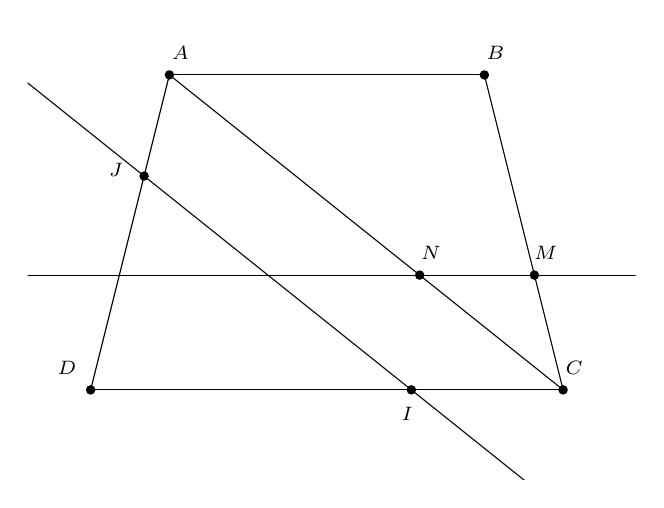
\begin{tikzpicture}[line cap=round,line join=round,>=triangle 45,x=1.0cm,y=1.0cm]
\clip(-3.8,-0.14) rectangle (3.92,5.6);
\draw (-2.,5.)-- (2.,5.);
\draw (2.,5.)-- (3.,1.);
\draw (3.,1.)-- (-3.,1.);
\draw (-3.,1.)-- (-2.,5.);
\draw (-2.,5.)-- (3.,1.);
\draw [domain=-3.8:3.92] plot(\x,{(-14.745365853658539-0.*\x)/-6.});
\draw [domain=-3.8:3.92] plot(\x,{(--9.291764705882354-4.*\x)/5.});
\begin{scriptsize}
\draw [fill=black] (-2.,5.) circle (1.5pt);
\draw[color=black] (-1.86,5.28) node {$A$};
\draw [fill=black] (2.,5.) circle (1.5pt);
\draw[color=black] (2.14,5.28) node {$B$};
\draw [fill=black] (3.,1.) circle (1.5pt);
\draw[color=black] (3.14,1.28) node {$C$};
\draw [fill=black] (-3.,1.) circle (1.5pt);
\draw[color=black] (-3.3,1.28) node {$D$};
\draw [fill=black] (1.1780487804878046,2.4575609756097565) circle (1.5pt);
\draw[color=black] (1.32,2.74) node {$N$};
\draw [fill=black] (2.6356097560975607,2.4575609756097565) circle (1.5pt);
\draw[color=black] (2.78,2.74) node {$M$};
\draw [fill=black] (-2.3211764705882354,3.715294117647059) circle (1.5pt);
\draw[color=black] (-2.68,3.8) node {$J$};
\draw [fill=black] (1.0729411764705885,1.) circle (1.5pt);
\draw[color=black] (1.02,0.7) node {$I$};
\end{scriptsize}
\end{tikzpicture}
\end{exo}

\begin{exo}
\begin{minipage}{0.4\linewidth}
\definecolor{cqcqcq}{rgb}{0.7529411764705882,0.7529411764705882,0.7529411764705882}
\begin{tikzpicture}[line cap=round,line join=round,>=triangle 45,x=1.0cm,y=1.0cm]
\clip(-3.74,0.06) rectangle (3.06,5.64);
\draw (-3.,1.)-- (2.,2.);
\draw (2.,2.)-- (-1.,5.);
\draw (-1.,5.)-- (-3.,1.);
\draw [domain=-3.74:3.06] plot(\x,{(-8.9-4.*\x)/-2.});
\begin{scriptsize}
\draw [fill=black] (2.,2.) circle (1.5pt);
\draw[color=black] (2.16,2.28) node {$A$};
\draw [fill=black] (-1.,5.) circle (1.5pt);
\draw[color=black] (-0.86,5.38) node {$B$};
\draw [fill=black] (-3.,1.) circle (1.5pt);
\draw[color=black] (-3.34,1.26) node {$C$};
\draw [fill=black] (-0.15,4.15) circle (1.5pt);
\draw[color=black] (0.12,4.26) node {$E$};
\draw [fill=black] (-1.5833333333333333,1.2833333333333334) circle (1.5pt);
\draw[color=black] (-1.44,1.02) node {$F$};
\end{scriptsize}
\end{tikzpicture}
\end{minipage}
\begin{minipage}{0.6\linewidth}
On considère la figure ci-contre tels que  $(EF) // (BC)$  et  $AF=x$ et $AE=x-1$ et $AC=9$ et $AB=7$
\begin{questions}
\question Calculer le nombre $x$.
\question Déduire que : $BC=2EF$.
\end{questions}
\end{minipage}
\end{exo}

\end{document}